\chapter{Opis problema}
\label{ch:opis-problema}
Ovaj rad bavi se problemom raspoznavanja studentskih identifikacijskih brojeva, poznatih pod skraćenicom
\emph{JMBAG}\footnote{\emph{Jedinstveni Matični Broj Akademskog Građana.}}. Ti brojevi se sastoje od deset znamenaka i
svakom studentu je dodijeljen jedinstveni broj koji služi kao identifikator studenta u sustavu hrvatskih fakulteta.
Kod pristupanja ispitima, od studenata se očekuje da uz ime i prezime također napišu svoj \emph{JMBAG} kako bi ih se
moglo jedinstveno identificirati u sustavu. Stoga je korisno napraviti sustav koji će moći automatski raspoznavati te
brojeve. Problem raspoznavanja \emph{JMBAG}-ova može se podijeliti u tri faze: pretprocesiranje, segmentacija i
klasifikacija. Faza pretprocesiranja služi kako bi se ulazna slika normirala te kako bi se znamenke odvojile od
pozadine. U fazi segmentacije potrebno je odrediti granice između pojedinačnih znamenki \emph{JMBAG}-a kako bi se svaka
znamenka mogla pojedinačno raspoznavati. Moguće je raspoznavati i više znamenki odjednom, ali tada klasifikator mora
biti kompleksniji i skup podataka za učenje mora biti veći. Zbog toga je poželjnije raspoznavati pojedinačne znamenke,
jer se skup za učenje efektivno poveća deset puta i sam klasifikator može biti jednostavniji. Posljednja faza
klasifikacije raspoznaje svaku znamenku pojedinačno. Slijednim spajanjem pojedinačno klasificiranih brojeva dobiva se
konačno raspoznati \emph{JMBAG}. U sljedećim odjeljcima bit će opisana implementacija navedenih faza raspoznavanja te
njihovo povezivanje u sustav za raspoznavanje \emph{JMBAG}-ova. Također će biti opisan način povezivanja navedenih faza
u konačan program kojim se trenira neuronska mreža i omogućuje raspoznavanje brojeva proizvoljnog broja znamenaka.
\newpage

\section{Pretprocesiranje}
\label{sec:pretprocesiranje}
Faza pretprocesiranja omogućuje jednoliko tretiranje ulaznih slika u preostalim fazama raspoznavanja. To se postiže na
način da se ulazna slika binarizira - dio slike koji predstavlja broj mora biti jasno odvojen od pozadine slike.
Slika\ \ref{fig:preprocessing-original-image} je primjer ulazne slike nekog \emph{JMBAG}-a.
\begin{figure}[!htb]
    \centering
    
\includegraphics[width=12cm]{images/chapter4/preprocessing-original-image.png}
    \caption{\emph{JMBAG} prije pretprocesiranja.}
    \label{fig:preprocessing-original-image}
\end{figure}
\newline
Nakon učitavanja slike u memoriju, prvi korak prema binarizaciji je uklanjanje svih boja iz slike. Time će se dobiti
slika u nijansama sive boje nad kojom se dalje može provesti postupak binarizacije. Kako bi se uklonila boja iz slike,
za svaki piksel računa se njegov intenzitet na sljedeći način:\\
\begin{equation}
    I = \left(\frac{I_{crvena} + I_{zelena} + I_{plava}}{765}\right)^{2} \cdot 255.\label{eq:pixel-intensity}
\end{equation}\\
Kako se piksel sastoji od komponenata $I_{crvena}$, $I_{zelena}$ i $I_{plava}$ čiji je raspon vrijednosti $[0, 255]$,
pri izračunu intenziteta njihov zbroj se dijeli sa zbrojem njihovih maksimalnih vrijednosti ($3 \cdot 255 = 765$).
Dobiveni rezultat se zatim kvadrira kako bi se bolje aproksimirala percepcija ljudskog oka na svjetlinu. Na kraju,
kvadrirani rezultat pomnoži se s $255$ kako bi se opet dobila vrijednost u rasponu $[0, 255]$. Dobiveni intenzitet $I$
zatim se koristi kao nova vrijednost komponenata $I_{crvena}$, $I_{zelena}$ i $I_{plava}$ za taj piksel. Opisani proces
uklanjanja boje prikazan je na slici\ \ref{fig:preprocessing-grayscale-image}.\\
\begin{figure}[!htb]
    \centering
    
\includegraphics[width=12cm]{images/chapter4/preprocessing-grayscale-image.png}
    \caption{\emph{JMBAG} nakon uklanjanja boje iz slike.}
    \label{fig:preprocessing-grayscale-image}
\end{figure}
\newpage
\noindent
Sada kada je za svaki piksel izračunat njegov intenzitet, može se provesti postupak binarizacije. Prvo je potrebno
pronaći minimalnu vrijednost intenziteta $I_{\min}$ i maksimalnu vrijednost intenziteta $I_{\max}$ na cijeloj slici za
sve potpuno vidljive piksele\footnote{Piksel se smatra potpuno vidljivim ako je vrijednost njegove neprozirnosti
jednaka $255$.}. Preko $I_{\min}$ i $I_{\max}$ računa se intenzitet odsijecanja:\\
\begin{equation}
    I_{o} = \frac{I_{\max} - I_{\min}}{2}.\label{eq:cutoff-intensity}
\end{equation}\\
Intenzitet odsijecanja $I_{o}$ zatim se koristi kako bi se slika binarizirala na sljedeći način:
\begin{enumerate}
    \item Ako je vrijednost neprozirnosti piksela $(x, y)$ manja od $255$, piksel će pripadati pozadini.
    \item Ako je intenzitet piksela $(x, y)$ veći od intenziteta odsijecanja $I_{o}$, piksel će pripadati pozadini.
    \item Inače će piksel pripadati \emph{JMBAG}-u koji se raspoznaje.
\end{enumerate}
Kod binarizacije pikseli pozadine su bijele boje, dok su pikseli \emph{JMBAG}-a crne boje.
Slika\ \ref{fig:preprocessing-binarized-image} prikazuje jedan \emph{JMBAG} nakon konačnog koraka pretprocesiranja.
\begin{figure}[htb]
    \centering
    
\includegraphics[width=12cm]{images/chapter4/preprocessing-binarized-image.png}
    \caption{\emph{JMBAG} nakon postupka binarizacije.}
    \label{fig:preprocessing-binarized-image}
\end{figure}
\newpage


\section{Segmentacija}
\label{sec:segmentacija}
Nakon binarizacije potrebno je pronaći granice među brojevima \emph{JMBAG}-a kako bi se mogli zasebno raspoznavati u
klasifikatoru. Kako slika dobivena postupkom binarizacije sadrži samo crnu i bijelu boju, za postupak segmentacije
korištena je pretpostavka da su brojevi na slici pojedinačno odvojene komponente. Stoga prvi korak segmentacije
pronalazi sve crne povezane komponente na slici te ih grupira u međusobno disjunktne skupove piksela koji će se u
daljnjem tekstu nazivati grupama piksela. U idealnom slučaju, svaka znamenka sastojat će se od samo jedne grupe piksela
koja je odvojena od svih ostalih grupa znamenaka, time ukupno tvoreći deset grupa piksela. Ovakav slučaj prikazan je na
slici\ \ref{fig:ideal-segmentation} gdje je svaka grupa piksela obojena različitom bojom.
\begin{figure}[htb]
    \centering
    
\includegraphics[width=12cm]{images/chapter4/ideal-segmentation.png}
    \caption{Idealno odvojene znamenke \emph{JMBAG}-a.}
    \label{fig:ideal-segmentation}
\end{figure}
\newline
Međutim, ovo neće uvijek biti slučaj te će neke slike sadržavati veći ili manji broj grupa piksela koje ne moraju nužno
odgovarati pojedinačnim znamenkama. Kako bi se za takve slike proveo postupak segmentacije, pronađene grupe piksela
dijele se na glavne i sporedne grupe piksela. Glavne grupe piksela čini skupina od najviše deset grupa piksela sa slike
koje pojedinačno sadrže barem $\frac{1}{30}$ ukupnog broja crnih piksela na slici, dok su sve ostale grupe sporedne
grupe. Time je osigurano da će glavnih grupa uvijek biti deset ili manje. Ovisno o broju pronađenih glavnih grupa,
implementirani algoritam segmentacije podešava skup glavnih grupa na način:
\begin{enumerate}
    \item Ako je pronađeno 10 glavnih grupa, skup glavnih grupa ne treba podešavati.
    \item Ako je pronađeno 9 glavnih grupa, glavna grupa najveće širine uklanja se iz skupa glavnih grupa te se dijeli
    na pola po širini. Time se dobivaju dvije nove grupe piksela koje se dodaju u skup glavnih grupa koji tada sadrži
    ukupno 10 grupa.
    \item Ako je pronađeno 8 glavnih grupa, dvije glavne grupe najveće širine uklanjaju se iz skupa glavnih grupa.
    Zatim se uspoređuje omjer širina najšire i druge najšire uklonjene grupe. Ako je taj omjer veći ili jednak $1{,}33$,
    najšira grupa dijeli se na tri jednaka dijela po širini te se tako dobivene grupe uz preostalu grupu dodaju u skup
    glavnih grupa. S druge strane, ako je omjer širina manji od $1{,}33$ obje uklonjene grupe dijele se na pola po
    širini te se novonastale grupe dodaju u skup glavnih grupa. U oba slučaja, skup glavnih grupa sadržavat će ukupno
    10 grupa.
    \item Ako je pronađeno 7 ili manje glavnih grupa, tada se $10 - n$ najširih grupa dijeli na pola po širini, gdje je
    $n$ broj pronađenih glavnih grupa.
\end{enumerate}
Ako nakon prethodnog koraka podešavanja skup glavnih grupa ne sadrži ukupno 10 grupa, algoritam segmentacije označava
sliku kao neispravnu te se postupak klasifikacije neće provoditi za tu sliku. U suprotnom, algoritam nastavlja s radom.
Slika\ \ref{fig:segmentation-division} prikazuje navedeni proces podešavanja glavnih grupa za slučaj 9 pronađenih
glavnih grupa. Stanje prije podešavanja glavnih grupa prikazuje najširu grupu označenu sivom bojom, dok su nakon
postupka podešavanja sve znamenke označene različitim bojama.
\begin{figure}[htb]
    \begin{subfigure}{\textwidth}
        \centering
        
\includegraphics[width=12cm]{images/chapter4/segmentation-before-division.png}
        \caption{Prije podešavanja.}
    \end{subfigure}
    \begin{subfigure}{\textwidth}
        \centering
        
\includegraphics[width=12cm]{images/chapter4/segmentation-after-division.png}
        \caption{Nakon podešavanja.}
    \end{subfigure}
    \caption{\emph{JMBAG} s dvije povezane znamenke prije i nakon podešavanja glavnih grupa piksela.}
    \label{fig:segmentation-division}
\end{figure}
\newline
Sljedeći korak jest pronaći kojim glavnim grupama teže pojedinačne sporedne grupe. Prvo se za svaku glavnu i sporednu
grupu računa središte $(x_s, y_s)$:\\
\begin{align}
    x_s = \frac{\sum_{n = 1}^{N} x_n}{N}\label{eq:x-center}\\
    y_s = \frac{\sum_{n = 1}^{N} y_n}{N}\label{eq:y-center}
\end{align}\\
gdje je $N$ broj crnih piksela u grupi. Za svako središte glavne grupe $(x_{s_g}, y_{s_g})$ i središte sporedne grupe
$(x_{s_s}, y_{s_s})$ računa se njihova međusobna \emph{Euklidska} udaljenost:\\
\begin{equation}
    D = \sqrt{(x_{s_g} - x_{s_s})^{2} + (y_{s_g} - y_{s_s})^{2}}\label{eq:euclidean-distance}
\end{equation}\\
te se svaka sporedna grupa pridjeljuje najbližoj glavnoj grupi. Nakon opisanog postupka postojat će 10 grupa piksela
na temelju kojih se svaka znamenka izdvaja u zasebnu sliku. Slika\ \ref{fig:assigned-minor-groups} prikazuje stanje
prije i nakon dodjeljivanja sporednih grupa (označenih crnom bojom) glavnim grupama.
\begin{figure}[htb]
    \begin{subfigure}{\textwidth}
        \centering
        
\includegraphics[width=12cm]{images/chapter4/unassigned-minor-groups.png}
        \caption{Prije dodjeljivanja.}
    \end{subfigure}
    \begin{subfigure}{\textwidth}
        \centering
        
\includegraphics[width=12cm]{images/chapter4/assigned-minor-groups.png}
        \caption{Nakon dodjeljivanja.}
    \end{subfigure}
    \caption{Glavne i sporedne grupe piksela prije i nakon postupka dodjeljivanja.}
    \label{fig:assigned-minor-groups}
\end{figure}
\newpage


\section{Klasifikacija}
\label{sec:klasifikacija}
Postupkom segmentacije binarizirana slika podijeljena je na pojedinačne slike od kojih svaka sadrži jednu znamenku. Kao
klasifikator korištena je unaprijedna neuronska mreža s fiksnim brojem ulaza i izlaza, pa je stoga potrebno ulazne slike
svesti na određen broj značajki. Primjer segmentiranih znamenaka prikazan je na slici\ \ref{fig:segmented}.
\begin{figure}[htb]
    \centering
    \frame{
\includegraphics[width=1cm]{images/chapter4/segmented-1.png}}
    \frame{
\includegraphics[width=1cm]{images/chapter4/segmented-2.png}}
    \frame{
\includegraphics[width=1cm]{images/chapter4/segmented-3.png}}
    \frame{
\includegraphics[width=1cm]{images/chapter4/segmented-4.png}}
    \frame{
\includegraphics[width=1cm]{images/chapter4/segmented-5.png}}
    \frame{
\includegraphics[width=1cm]{images/chapter4/segmented-6.png}}
    \frame{
\includegraphics[width=1cm]{images/chapter4/segmented-7.png}}
    \frame{
\includegraphics[width=1cm]{images/chapter4/segmented-8.png}}
    \frame{
\includegraphics[width=1cm]{images/chapter4/segmented-9.png}}
    \frame{
\includegraphics[width=1cm]{images/chapter4/segmented-0.png}}
    \caption{Pojedinačne slike znamenaka nakon segmentiranja.}
    \label{fig:segmented}
\end{figure}
\newline
Segmentirane slike su različitih dimenzija te njihov omjer visine i širine nije uvijek $1:1$. Također se crni pikseli
nalaze na samom rubu svake slike. Stoga se segmentirane slike nadopunjavaju na način:
\begin{enumerate}
    \item Ako je visina slike veća od njene širine, slici se s lijeve i desne strane dodaju stupci bijelih piksela sve
    dok širina i visine nisu jednake.
    \item Ako je visina slike manja od njene širine, slici se s gornje i donje strane dodaju redovi bijelih piksela
    sve dok širina i visina slike nisu jednake.
\end{enumerate}
Nakon nadopunjavanja slika će uvijek imati omjer širine i visine jednak $1:1$, kao što je prikazano na
slici\ \ref{fig:scaled}.
\begin{figure}[htb]
    \centering
    \frame{
\includegraphics[width=1cm]{images/chapter4/scaled-1.png}}
    \frame{
\includegraphics[width=1cm]{images/chapter4/scaled-2.png}}
    \frame{
\includegraphics[width=1cm]{images/chapter4/scaled-3.png}}
    \frame{
\includegraphics[width=1cm]{images/chapter4/scaled-4.png}}
    \frame{
\includegraphics[width=1cm]{images/chapter4/scaled-5.png}}
    \frame{
\includegraphics[width=1cm]{images/chapter4/scaled-6.png}}
    \frame{
\includegraphics[width=1cm]{images/chapter4/scaled-7.png}}
    \frame{
\includegraphics[width=1cm]{images/chapter4/scaled-8.png}}
    \frame{
\includegraphics[width=1cm]{images/chapter4/scaled-9.png}}
    \frame{
\includegraphics[width=1cm]{images/chapter4/scaled-0.png}}
    \caption{Pojedinačne znamenke nakon ujednačavanja visine i širine.}
    \label{fig:scaled}
\end{figure}
Takva slika nadopunjava se još jednom sa svake strane tako da se dodaje obrub bijelih piksela. Obrub će povećati visinu
i širinu slike sa svake strane za $20\%$, tako de će se ukupna visina i širina slike povećati za $40\%$ što je prikazano
na slici\ \ref{fig:padding}.
\begin{figure}[htb]
    \centering
    \frame{
\includegraphics[width=1cm]{images/chapter4/padding-1.png}}
    \frame{
\includegraphics[width=1cm]{images/chapter4/padding-2.png}}
    \frame{
\includegraphics[width=1cm]{images/chapter4/padding-3.png}}
    \frame{
\includegraphics[width=1cm]{images/chapter4/padding-4.png}}
    \frame{
\includegraphics[width=1cm]{images/chapter4/padding-5.png}}
    \frame{
\includegraphics[width=1cm]{images/chapter4/padding-6.png}}
    \frame{
\includegraphics[width=1cm]{images/chapter4/padding-7.png}}
    \frame{
\includegraphics[width=1cm]{images/chapter4/padding-8.png}}
    \frame{
\includegraphics[width=1cm]{images/chapter4/padding-9.png}}
    \frame{
\includegraphics[width=1cm]{images/chapter4/padding-0.png}}
    \caption{Segmentiranje znamenke nakon konačnog postupka nadopunjavanja.}
    \label{fig:padding}
\end{figure}
Dimenzije slika nakon konačnog postupka nadopunjavanja i dalje nisu jednake za sve slike, te se stoga značajke odabiru
tako da se računaju udaljenosti do prvog crnog piksela počevši od nekog ruba slike. Također se računaju udaljenosti do
prvog crnog piksela počevši od središta slike. Ove udaljenosti prikazane su na
slici\ \ref{fig:features-for-single-digit} za jednu znamenku te na slici\ \ref{fig:features-for-multiple-digits} za svih
10 znamenaka. Na obje slike udaljenosti su označene različitim bojama na sljedeći način:
\begin{enumerate}
    \item Udaljenosti od vrha i dna slike za 6 jednoliko udaljenih stupaca označene su crvenom bojom.
    \item Udaljenosti s lijeve i desne strane slike za 6 jednoliko udaljenih redaka označene su plavom bojom.
    \item Dijagonalne udaljenosti sa sva 4 ruba slike označene su ljubičastom bojom.
    \item Udaljenosti od središta slike prema gore, dolje, lijevo, desno te po 4 dijagonale označene su zelenom bojom.
\end{enumerate}
\begin{figure}[htb]
    \centering
    \frame{
\includegraphics[width=5cm]{images/chapter4/features-0.png}}
    \caption{Značajke za jednu znamenku \emph{JMBAG}-a.}
    \label{fig:features-for-single-digit}
\end{figure}
\begin{figure}[htb]
    \centering
    \frame{
\includegraphics[width=1cm]{images/chapter4/features-1.png}}
    \frame{
\includegraphics[width=1cm]{images/chapter4/features-2.png}}
    \frame{
\includegraphics[width=1cm]{images/chapter4/features-3.png}}
    \frame{
\includegraphics[width=1cm]{images/chapter4/features-4.png}}
    \frame{
\includegraphics[width=1cm]{images/chapter4/features-5.png}}
    \frame{
\includegraphics[width=1cm]{images/chapter4/features-6.png}}
    \frame{
\includegraphics[width=1cm]{images/chapter4/features-7.png}}
    \frame{
\includegraphics[width=1cm]{images/chapter4/features-8.png}}
    \frame{
\includegraphics[width=1cm]{images/chapter4/features-9.png}}
    \frame{
\includegraphics[width=1cm]{images/chapter4/features-0.png}}
    \caption{Značajke za svih 10 znamenaka \emph{JMBAG}-a.}
    \label{fig:features-for-multiple-digits}
\end{figure}
Na ovaj način dobiveno je ukupno 36 udaljenosti koje se skaliraju na raspon $[0, 1]$ koristeći visinu i širinu slike.
Ovako skalirane udaljenosti koriste se kao značajke koje su ulaz unaprijedne neuronske mreže. Broj skrivenih slojeva
neuronske mreže nije fiksan te se može podešavati kod postupka učenja, što je opisano u idućem odjeljku. Neuronska
mreža ima ukupno deset izlaza, jedan za svaku znamenku u rasponu $[0, 9]$. Vrijednosti svakog od izlaza su uvijek u
rasponu $[0, 1]$ te se stoga izlazi mreže mogu smatrati kao vjerojatnosti da ulazi predstavljaju svaku od znamenki. Da
bi se odredila klasifikacija neke znamenke, uzima se vrijednost najvećeg izlaza mreže te se znamenka dodijeljena tom
izlazu uzima kao klasifikacija ulazne znamenke.


\section{Implementacija sustava za raspoznavanje}
\label{sec:implementacija-sustava-za-raspoznavanje}
Prethodno opisane faze zajedno čine sustav za raspoznavanje \emph{JMBAG}-ova. Sustav je implementiran kao jedinstven
program koji nudi mogućnost treniranja neuronske mreže, testiranja točnosti istrenirane neuronske mreže, mogućnost
odvojenog pretprocesiranja, segmentiranja i odabira značajki kako bi se izbjeglo ponavljano učitavanje istih slika, te
mogućnost raspoznavanja pojedinih slika. Funkcija programa odabire se pri njegovom pokretanju preko argumenata
naredbenog retka. Kao prvi argument program očekuje željenu funkciju:
\begin{enumerate}
    \item Za funkciju odvojenog pretprocesiranja, segmentiranja i odabira značajki prvi argument mora biti
    \texttt{prepare}.
    \item Za funkciju treniranja neuronske mreže prvi argument mora biti \texttt{train}.
    \item Za funkciju testiranja neuronske mreže prvi argument mora biti \texttt{test}.
    \item Za funkciju raspoznavanja pojedinih slika prvi argument mora biti \texttt{apply}.
\end{enumerate}

\subsection{Funkcija \texttt{prepare}}
\label{subsec:funkcija-prepare}
Ova funkcija nudi mogućnost odvojene obrade slika u svrhu bržeg učitavanja kod postupka treniranja. Pri pokretanju
programa koristeći ovu funkciju nad ulaznim slikama bit će obavljen postupak pretprocesiranja, segmentacije i odabira
značajki te će pronađene značajke i labele biti spremljene u navedenu datoteku u tekstualnom formatu\footnote{Primjer
zapisa značajki u ovom formatu dostupan je u
dodatku\ \ref{ch:primjer-serijaliziranih-podataka-znacajki-slike-i-neuronske-mreze}.}.
Slika\ \ref{fig:prepare-diagram} prikazuje blok-dijagram implementacije funkcije \texttt{prepare}, dok
tablica\ \ref{tab:prepare-args} opisuje dostupne argumente te funkcije.
\begin{table}[htb]
    \caption{Argumenti funkcije \texttt{prepare}.}
    \label{tab:prepare-args}
    \scriptsize
    \centering
    \begin{tabular}{|M{3.5cm}|M{2.5cm}|M{6cm}|}
        \hline
        Argument & Tip & Opis \\
        \hline
        \texttt{-{}-images \underline{DIR}} & Direktorij & Obavezan argument koji specificira direktorij
        \texttt{\underline{DIR}} u kojem se nalaze slike znamenaka. Labela slike očekuje se u prvih
        \texttt{\underline{N}} znakova imena slike, gjde je \texttt{\underline{N}} određen argumentom
        \texttt{-{}-n-per-image}. \\
        \hline
        \texttt{-{}-n-per-image \underline{N}} & Pozitivan cijeli broj & Neobavezan argument koji specificira broj
        znamenaka \texttt{\underline{N}} koji se nalazi na svakoj od ulaznih slika. Ako ovaj argument nije naveden,
        pretpostavljena vrijednost je $10$ znamenaka po slici. \\
        \hline
        \texttt{-{}-output \underline{DAT}} & Datoteka & Obavezan argument koji specificira izlaznu datoteku
        \texttt{\underline{DAT}} u koju će biti spremljeni serijalizirani podatci o značajkama ulaznih slika. \\
        \hline
        \texttt{-{}-debug \underline{DIR}} & Direktorij & Neobavezan argument koji specificira direktorij
        \texttt{\underline{DIR}} u koji će biti spremljene slike koraka pretprocesiranja, segmentacije i odabira
        značajki. \\
        \hline
    \end{tabular}
\end{table}
\begin{figure}[htb]
    \centering
    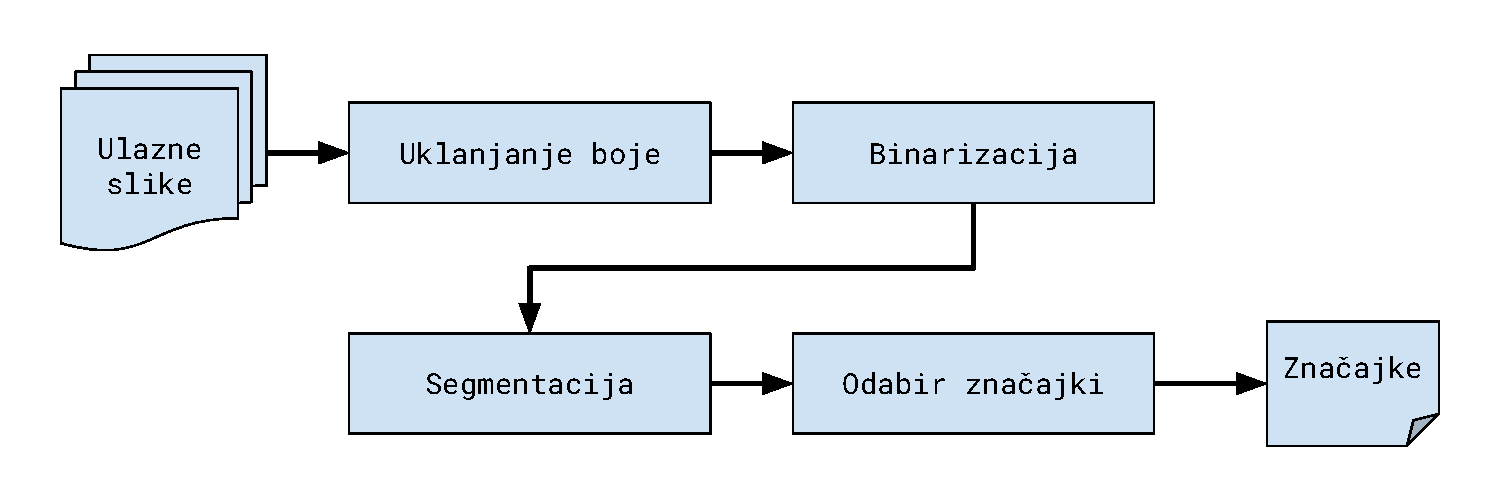
\includegraphics[width=12cm]{images/chapter4/prepare-diagram.pdf}
    \caption{Blok-dijagram funkcije \texttt{prepare}.}
    \label{fig:prepare-diagram}
\end{figure}

\subsection{Funkcija \texttt{train}}
\label{subsec:funkcija-train}
Od sve četiri dostupne funkcije, funkcija \texttt{train} je najkompleksnija i nudi najveći opseg različitih opcija pri
pokretanju. Zadatak ove funkcije je učitati sirove slike ili tekstualne značajke slika te koristeći njih trenirati
novu ili postojeću neuronsku mrežu. Kod stvaranja nove neuronske mreže, težinski faktori bit će inicijalizirani na
nasumične vrijednosti u rasponu $[-0.4, 0.4]$ dok će neuronska mreža uvijek imati ulazni sloj veličine $36$, izlazni
sloj veličine $10$, te proizvoljan broj i dimenzije skrivenih slojeva. Argumenti koji određuju hoće li se koristiti
slike ili tekstualne značajke te hoće li se trenirati nova ili postojeća mreža opisani su u
tablici\ \ref{tab:train-args-1}.
\begin{table}[htb]
    \caption{Argumenti funkcije \texttt{train} za podešavanje ulaznih slika i neuronske mreže.}
    \label{tab:train-args-1}
    \scriptsize
    \centering
    \begin{tabular}{|M{3.5cm}|M{2.5cm}|M{6cm}|}
        \hline
        Argument & Tip & Opis \\
        \hline
        \texttt{-{}-images \underline{DIR}} & Direktorij & Argument koji specificira direktorij \texttt{\underline{DIR}}
        u kojem se nalaze slike znamenaka koje će se koristiti za treniranje neuronske mreže. Labela slike očekuje se u
        prvih \texttt{\underline{N}} znakova imena slike, gjde je \texttt{\underline{N}} određen argumentom
        \texttt{-{}-n-per-image}. \\
        \hline
        \texttt{-{}-n-per-image \underline{N}} & Pozitivan cijeli broj & Neobavezan argument koji specificira broj
        znamenaka \texttt{\underline{N}} koji se nalazi na svakoj od ulaznih slika. Ako ovaj argument nije naveden,
        pretpostavljena vrijednost je $10$ znamenaka po slici. Vrijednost ovog argumenta koristi se samo u slučaju kada
        je specificiran argument \texttt{-{}-images}. \\
        \hline
        \texttt{-{}-features \underline{DIR}} & Direktorij & Argument koji specificira direktorij
        \texttt{\underline{DIR}} u kojem se nalaze serijalizirane značajke koje će se koristiti za treniranje neuronske
        mreže. \\
        \hline
        \texttt{-{}-load \underline{DAT}} & Datoteka & Argument koji specificira datoteku \texttt{\underline{DAT}} u
        kojoj se nalazi serijalizirani opis neuronske mreže koju treba trenirati. \\
        \hline
        \texttt{-{}-layout \underline{STR}} & Niz pozitivnih cijelih brojeva odvojenih znakom \emph{`x'} &
        Neobavezan argument koji specificira strukturu \texttt{\underline{STR}} skrivenih slojeva neuronske mreže.
        Dimenzije skrivenih slojeva odvojene su znakom \emph{`x'}. Ako ovaj argument nije naveden, njegova
        pretpostavljena vrijednost je \emph{``10x10''}. Ako je naveden argument \texttt{-{}-load}, ovaj argument bit će
        zanemaren. \\
        \hline
    \end{tabular}
\end{table}
Pri pokretanju naredbe \texttt{train} obavezno je navesti argument \texttt{-{}-images} ili argument
\texttt{-{}-features}. Ako su navedena oba argumenta, bit će korištena vrijednost argumenta koji je naveden posljednji u
nizu. Naredba \texttt{train} također nudi argumente za podešavanje algoritma \emph{Backpropagation} koji se koristi za
treniranje neuronske mreže koji su navedeni u tablici\ \ref{tab:train-args-2}.
\begin{table}[htb]
    \caption{Argumenti funkcije \texttt{train} za podešavanje algoritma \emph{Backpropagation}.}
    \label{tab:train-args-2}
    \scriptsize
    \centering
    \begin{tabular}{|M{3.5cm}|M{2.5cm}|M{6cm}|}
        \hline
        Argument & Tip & Opis \\
        \hline
        \texttt{-{}-step \underline{$\eta$}} & Broj & Neobavezan argument koji specificira stopu učenja
        \texttt{\underline{$\eta$}} koja će se koristiti. Ako ovaj argument nije naveden, njegova pretpostavljena
        vrijednost je $1$. \\
        \hline
        \texttt{-{}-batch-size \underline{N}} & Pozitivan cijeli broj ili znakovni niz \emph{``all''} & Neobavezan
        argument koji specificira broj uzoraka za učenje \texttt{\underline{N}} koji će se koristiti u svakoj epohi
        algoritma. Umjesto broja moguće je navesti znakovni niz \emph{``all''} koji specificira da se koriste svi
        dostupni uzorci iz skupa za učenje u svakoj epohi algoritma. Ako ovaj argument nije naveden, njegova
        pretpostavljena vrijednost je \emph{``all''}. \\
        \hline
        \texttt{-{}-max-iters \underline{N}} & Pozitivan cijeli broj & Neobavezan argument koji specificira maksimalan
        broj epoha \texttt{\underline{N}} koji će algoritam izvršiti. Ako ovaj argument nije naveden, njegova
        pretpostavljena vrijednost je $10000$. \\
        \hline
        \texttt{-{}-target-error \underline{E}} & Broj & Neobavezan argument koji specificira stopu greške
        \texttt{\underline{E}} nakon koje će se algoritam zaustaviti. Ako ovaj argument nije naveden, njegova
        pretpostavljena vrijednost je $10^{-7}$. \\
        \hline
        \texttt{-{}-inertia \underline{$\alpha$}} & Broj & Neobavezan argument koji specificira koeficijent inercije
        \underline{$\alpha$}. Ako ovaj argument nije naveden, njegova pretpostavljena vrijednost je $0$. \\
        \hline
    \end{tabular}
\end{table}
Također je moguće dodati kriterij zaustavljanja učenja pri porastu greške na ispitnom skupu koristeći argumente opisane
u tablici\ \ref{tab:train-args-3}. Argumenti \texttt{-{}-test-images} i \texttt{-{}-test-features} su međusobno
isključivi kao argumenti \texttt{-{}-images} i \texttt{-{}-features} te će biti korišten samo argument koji je naveden
posljednji u nizu. Uz sve do sada navedene argumente dostupna su još dva argumenta: \texttt{-{}-output} i
\texttt{-{}-debug}. Argument \texttt{-{}-output} očekuje putanju datoteke u koju će biti spremljena serijalizirana
neuronska mreža dok je argument \texttt{-{}-debug} isti kao kod funkcije \texttt{prepare}, ali će se koristiti samo ako
je specificiran argument \texttt{-{}-images}. Na slici\ \ref{fig:train-diagram} prikazan je blok-dijagram funkcije
\texttt{train} bez dijela za učitavanje slika ispitnog skupa, koji je isti kao dio za učitavanje slika skupa za
treniranje.
\begin{table}[!htb]
    \caption{Argumenti funkcije \texttt{train} za podešavanje kriterija zaustavljanja pri porastu greške na ispitnom
    skupu.}
    \label{tab:train-args-3}
    \scriptsize
    \centering
    \begin{tabular}{|M{3.9cm}|M{2.1cm}|M{6cm}|}
        \hline
        Argument & Tip & Opis \\
        \hline
        \texttt{-{}-test-images \underline{DIR}} & Direktorij & Neobavezan argument koji specificira direktorij
        \texttt{\underline{DIR}} u kojem se nalaze slike ispitnog skupa. Ovaj argument koristi vrijednost argumenta
        \texttt{-{}-n-per-image} kao broj znamenaka na svakoj slici u ispitnom skupu. \\
        \hline
        \texttt{-{}-test-features \underline{DIR}} & Direktorij & Neobavezan argument koji specificira direktorij
        \texttt{\underline{DIR}} u kojem se nalaze serijalizirane značajke ispitnog skupa. \\
        \hline
        \texttt{-{}-test-moving-average \underline{N}} & Pozitivan cijeli broj & Neobavezan argument koji specificira
        broj zadnjih \texttt{\underline{N}} epoha algoritma za koje će se računati prosječna greška na ispitnom skupu.
        Kada izračunata prosječna greška počne rasti, algoritam prekida s radom. Ako ovaj argument nije naveden, njegova
        pretpostavljena vrijednost je $1$. \\
        \hline
    \end{tabular}
\end{table}
\begin{figure}[!htb]
    \centering
    \includegraphics[width=12cm]{images/chapter4/train-diagram.pdf}
    \caption{Blok-dijagram funkcije \texttt{train}.}
    \label{fig:train-diagram}
\end{figure}
\newpage

\subsection{Funkcija \texttt{test}}
\label{subsec:funkcija-test}
Funkcija \texttt{test} služi kako bi se provjerila točnost naučene neuronske mreže. Kod pokretanja programa koristeći
ovu funkciju može se navesti jedna ili više neuronskih mreža za koje će se provjeravati točnost na zadanom ispitnom
skupu. Ispitni skup zadaje se preko argumenta \texttt{-{}-images} uz argument \texttt{-{}-n-per-image} ili preko
argumenta \texttt{-{}-features}, koji se zadaju na isti način kako je opisano za funkciju \texttt{train}\footnote{
Također je dostupan i argument \texttt{-{}-debug} na isti način kao i kod funkcije \texttt{train}.}. Neuronske mreže
koje je potrebno testirati zadaju se preko argumenta \texttt{-{}-nn-paths} koji očekuje jednu ili više datoteka koje
sadrže neuronske mreže. Zbog toga argument \texttt{-{}-nn-paths} mora biti naveden zadnji u nizu. Ako su navedeni samo
ispitni podatci i neuronske mreže, funkcija \texttt{test} ispisat će samo postotak točnih klasifikacija na ispitnom
skupu pojedinačno za svaku od navedenih neuronskim mreža. Tablica\ \ref{tab:test-args} navodi argumente funkcije
\texttt{train} koji nude dodatne mogućnosti pri testiranju neuronskih mreža. Primjeri ispisa ove funkcije dostupni su u
dodatku\ \ref{ch:primjeri-ispisa-funkcije-test}.

\begin{table}[!htb]
    \caption{Argumenti funkcije \texttt{test} koji nude dodatne mogućnosti pri testiranju.}
    \label{tab:test-args}
    \scriptsize
    \centering
    \begin{tabular}{|M{3.5cm}|M{8.5cm}|}
        \hline
        Argument & Opis \\
        \hline
        \texttt{-{}-detail-by-number} & Kada je ovaj argument naveden ispis funkcije \texttt{test} će uključivati
        postotke točnih i pogrešnih klasifikacija za svaku od 10 znamenaka koje se raspoznaju. Ova statistika bit će
        ispisana zasebno za svaku od navedenih neuronskih mreža, osim ako je naveden argument \texttt{-{}-ensemble}. \\
        \hline
        \texttt{-{}-print-misses} & Navođenjem ovog argumenta bit će ispisane sve pogrešne klasifikacije svih ispitnih
        primjera uz ime datoteke ispitnog primjera. Ova statistika bit će ispisana zasebno za svaku od navedenih
        neuronskih mreža, osim ako je naveden argument \texttt{-{}-ensemble}. \\
        \hline
        \texttt{-{}-ensemble} & Ovaj argument će kombinirati sve navedene neuronske mreže u jedan klasifikator tako da
        se izlazi svih neuronskih mreža međusobno zbrajaju. Kada je ovaj argument naveden sve ostale statistike bit će
        ispisane samo jednom, kao da je navedena samo jedna neuronska mreža. \\
        \hline
    \end{tabular}
\end{table}

\subsection{Funkcija \texttt{apply}}
\label{subsec:funkcija-apply}
Ovo je najjednostavnija funkcija programa koja omogućuje raspoznavanje znamenaka na navedenim ulaznim slikama koristeći
odabranu neuronsku mrežu. Funkcija će za svaku od navedenih slika ispisati njeno ime i klasifikaciju brojeva na njoj
ako je moguće ispravno provesti proces segmentacije znamenaka. Već ranije opisan argument \texttt{-{}-n-per-image}
određuje broj znamenaka na svakoj slici, argument \texttt{-{}-nn-paths} određuje\hfill{}putanje\hfill{}do\hfill{}
datoteka\hfill{}koje\hfill{}sadrže\hfill{}opise\hfill{}neuronskih mreža dok\hfill{}argument\break\texttt{-{}-images}
specificira direktorij u kojem se nalaze slike koje treba raspoznati. Kako argument \texttt{-{}-nn-paths} očekuje jednu
ili više putanja do datoteka, on treba biti naveden posljednji u nizu argumenata. Mreže koje su navedene ovim argumentom
bit će kombinirane u jedan klasifikator zbrajanjem njihovih izlaznih vrijednosti.
